\label{section:hexacopter_design}

% {\color{red}Decision matrices and textual motivations for hardware choices and hardware system design will be added.}

The most commonly pictured multirotor drone is typically a quadcopter. A hexacopter, as opposed to a quadcopter, was chosen as the drone type for this project. The hexacopter design's 6 rotors allow for redundancy in the case of motor failure, it has a higher load capacity than an equivalent quadcopter, and its extra thrust and weight give it more control in strong wind. Closed drone systems, such as many of the DJI models, function as ``black boxes'' which is a problem in this case, since the goal is to develop a system which interacts with the flight controller. Therefore, only drone models which are highly configurable have been considered. 

\subsection{Basic Drone Hardware Requirements}

The specific drone model to be used was chosen based on the following factors:
\begin{itemize}
    \item \textbf{Flight Time} \\ Longer flight times obviously permit more testing, which is preferable. Having to recharge batteries between flights also means more flights are required for testing, and overhead time increases.
    \item \textbf{Load Capacity} \\ Higher load capacities allow the drone to carry instruments or cameras for later experiments, so that the drone is not only useful in the context of this project.
    \item \textbf{Cost} \\ Financial constraints always pose an issue to real-world testing, especially in the context of drone flight in rough weather, where parts may wear out quickly or crashes may occur. Initial cost should be minimized in order to permit replacement and additional purchases of parts.
    \item \textbf{Availability of Parts} \\ The parts used must be in continuous manufacture in order to ensure that the drone can still be used in the event of component failure.
    % \item \textbf{Model Reputation} \\ The drone must have good reviews from previous users. The goal of this project is not to test a specific drone platform, but rather only the landing system, so the performance of the drone itself should not be a major factor influencing the evaluation of the landing system.
\end{itemize}

\subsubsection{Drone System Comparison}

Multiple drone platforms have been considered for the physical migration of this landing system. Although it is infeasible and unnecessary to consider all drone models on the market, Table \ref{table:drone_system_ratings} outlines the main deciding factors in choosing among an existing 600-size hexacopter system, and two popular kits of similar size - the Tarot 680 Pro and the Hobby Power F550. The main issue with the existing hexacopter is that it is a few years old. Although it uses the well-reviewed DJI E600 propulsion system, this system is no longer in manufacture by DJI. This means that, if one of the motors or speed controllers fails, it would likely be better to replace all of them for consistency. The Tarot 680 Pro and Hobby Power F550 are also well-reviewed in online stores, and come in bundles with all necessary propulsion components which are affordable. Flight times of the models are those which use standard hardware setups with no loads. Load capacities are taken from the specifications given for each model.\footnote{DJI E600 Specs: \url{https://www.dji.com/e600/spec_v1-doc}}\footnote{Tarot 680 Specs: \url{http://www.helipal.com/tarot-fy680-pro-hexacopter-frame-set.html}} When the specifications are not supplied, estimates are derived from the performance of typical components that are used with the models. Such is the case with the estimated flight time and load capacity of the Hobby Power F550 with recommended Emax MT2213 motors.\footnote{Emax MT2213 specs: \url{https://www.rcmoment.com/p-rm4532.html}} The listed price is the typical price of the drone frame as well as a set of typical motors and speed controllers.

\begin{table}[ht]
    \centering
    \resizebox{\textwidth}{!}{
    \begin{tabular}{|p{5cm}|c|c|c|c|c|} \hline
    \textbf{Model} & \textbf{Flight Time (min)} & \textbf{Load Capacity (kg)} & \textbf{Base Cost (US\$)} & \textbf{Parts Availability} \\\hline
        \textbf{Current Hexacopter} & 30 & 2.5 & 0 & No \\\hline
        \textbf{Tarot 680 Pro} & 30 & 2.5 & 320 & Yes \\\hline
        \textbf{Hobby Power F550} & 20 & 2.0 & 170 & Yes \\\hline
    \end{tabular}
    }
    \caption{Drone System Comparison}
    \label{table:drone_system_ratings}
\end{table}

The \$0 cost of the current hexacopter system is misleading, as the fact that the propulsion system is discontinued may mean that unintended costs are quite high - comparable to the cost of building another drone. The HobbyPower F550's smaller size means that it is intended for 11.1 V batteries, decreasing overall load capacity and flight time.

Table \ref{tab:decision_matrix} shows a decision matrix for the selection of one of the considered drone models. Flight time and availability of parts are the factors that are weighted the highest, although load capacity and base cost are also considered. Of course, such a decision is not an exact science, and the variety of available parts influences both price and performance. This is an estimate, but provides a reasonable justification for the choice of drone model. The current hexacopter is not chosen mostly because of its age and inherent lack of available corresponding parts, although it does provide good flight time and load capacity. The Hobby Power F550 is cheap, but does not as much flight time as the other models, and has a lighter load capacity. The Tarot 680 Pro provides adequate flight time and load capacity, as well as a combo which is designed and rated for the given performance. These facts, as well as the fact that its price (including motors and speed controllers), is relatively affordable, also make it possible to create 2 usable drones. These drones will be identical except for differing flight controller setups, as outlined in Section \ref{section:flight_controllers}.

\begin{table}[ht]
    \centering
    \begin{tabular}{|c|c|c|c|c|}
    \hline
        \textbf{Factor} & \textbf{Weight} & \textbf{Current Hexacopter} & \textbf{Tarot 680} & \textbf{Hobby Power F550} \\\hline
        \textbf{Flight Time} & 0.4 & 5 & 5 & 3 \\\hline
        \textbf{Load Capacity} & 0.1 & 5 & 4 & 3 \\\hline
        \textbf{Base Cost} & 0.2 & 5 & 2 & 4 \\\hline
        \textbf{Parts Availability} & 0.3 & 0 & 5 & 5 \\\hline
        \textbf{Total} & 1.0 & 3.5 & 4.3 & 3.8 \\\hline
    \end{tabular}
    \caption{Decision matrix for the possible drone systems.}
    \label{tab:decision_matrix}
\end{table}

\subsection{Selected Components}

\begin{itemize}
    
    \item \textbf{Airframe:} Tarot 680 Pro, as shown in Figure \ref{subfig:tarot_680_pro} and \ref{subfig:tarot_680_pro_folded}. This is a 695 mm diameter, carbon fiber drone frame with arms and landing skids that fold to make the drone more portable. It is rated for 6 kg of thrust (with about 2.5 kg payload) using 22.2 V batteries and 330 mm propellers. The final diameter of the drone is thus 1025 mm.

    % \begin{figure}[ht]
    %     \centering
    %     \subfloat[The airframe expanded.]{{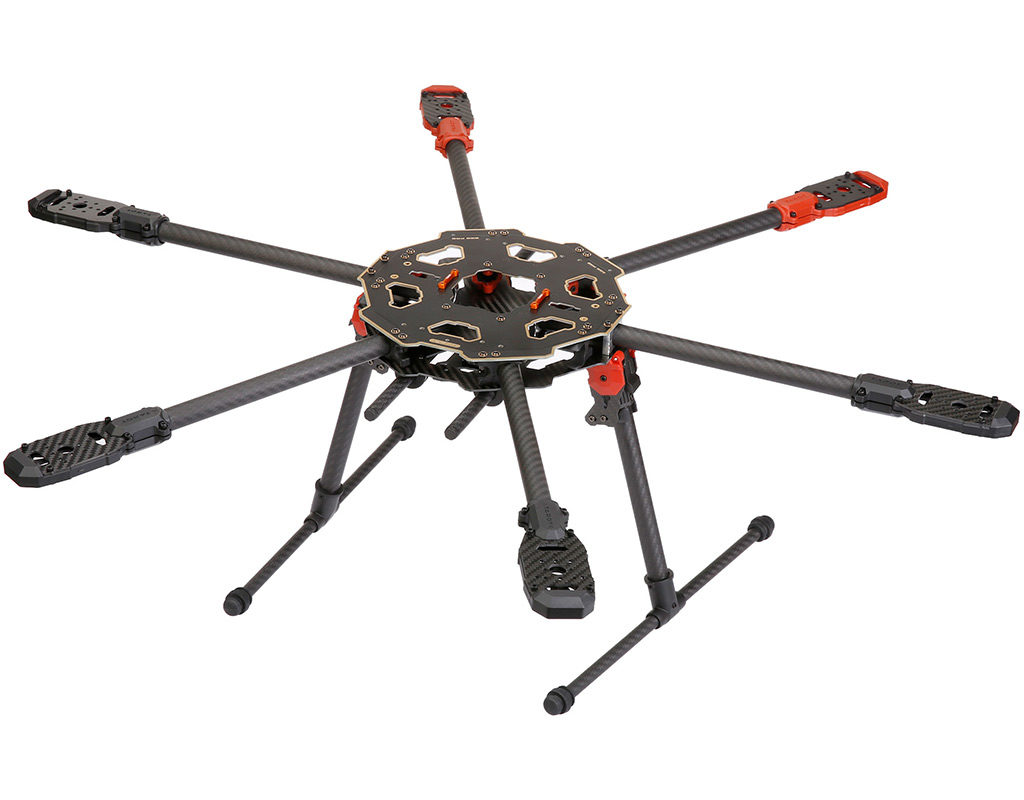
\includegraphics[width=0.3\textwidth]{images/tarot_680_pro.jpg}}} % http://www.alpha-rc-heli.com/shop/tarot-680-pro-hexacopter-kit/
    %     \hspace{2cm}
    %     \subfloat[The airframe folded.]{{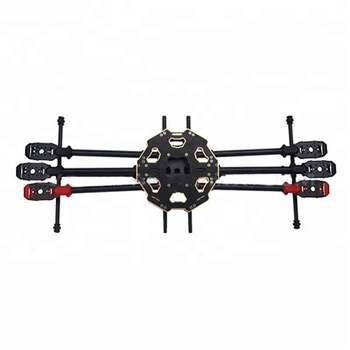
\includegraphics[width=0.3\textwidth]{images/tarot_680_pro_folded.jpg}}}
    %     \caption{The Tarot 680 Pro Airframe.} % https://www.alibaba.com/product-detail/TAROT-680PRO-Six-axis-Aircraft-Frame_1979377157.html
    %     \label{fig:tarot_680_pro}
    % \end{figure}

    \begin{figure}[ht]
        \centering
        \begin{subfigure}[b]{0.3\textwidth}
            \centering
            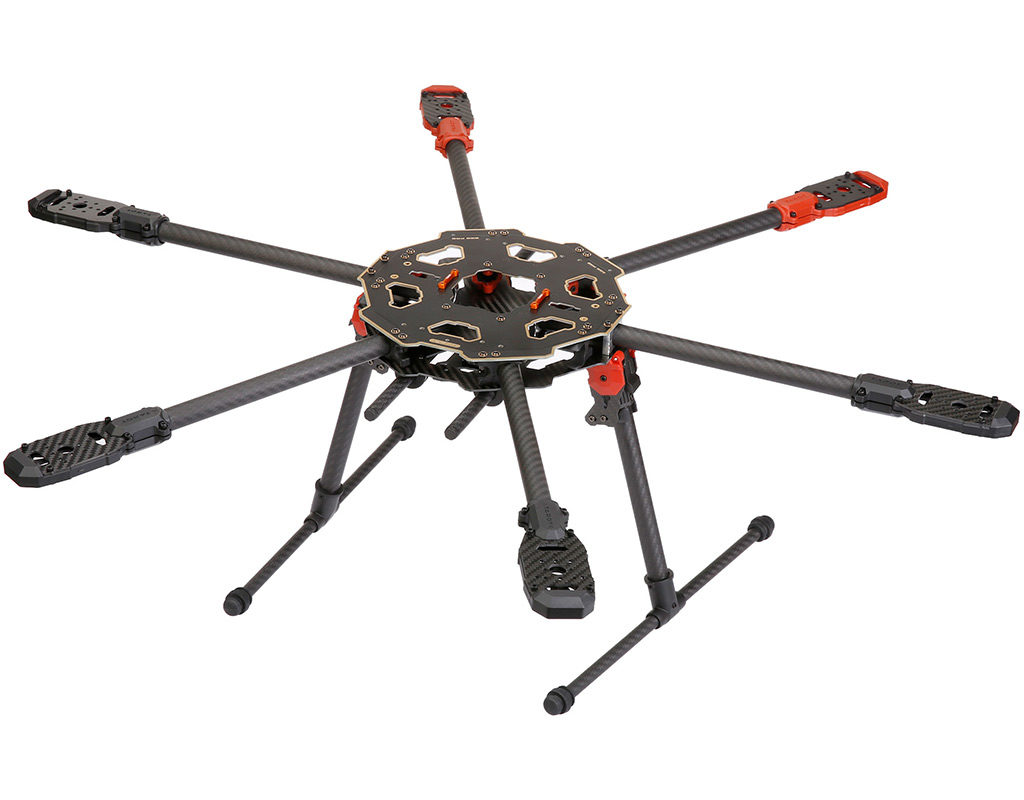
\includegraphics[width=\textwidth]{images/tarot_680_pro.jpg}
            \caption{The airframe expanded.}
            \label{subfig:tarot_680_pro}
        \end{subfigure}
        \hspace{2cm}
        \begin{subfigure}[b]{0.3\textwidth}
            \centering
            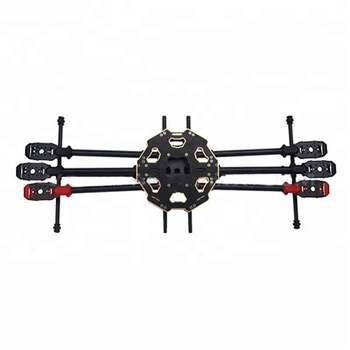
\includegraphics[width=\textwidth]{images/tarot_680_pro_folded.jpg}
            \caption{The airframe folded.}
            \label{subfig:tarot_680_pro_folded}
        \end{subfigure}
        \caption[The Tarot 680 Pro Airframe.]{The Tarot 680 Pro Airframe.\footnotemark}
        \label{fig:tarot_680_pro}
    \end{figure}
    \footnotetext{Image source: \url{http://www.alpha-rc-heli.com/shop/tarot-680-pro-hexacopter-kit/}}

    \item \textbf{Motors:} Tarot 4108 (380 kv), as recommended by the model package. These are the recommended motors for the model, with a diameter of $40.6 \approx 41$ mm and stator height of $8$ mm, comprising the ``4108'' model number. They are rated for 22.2 V batteries.

    \item \textbf{Speed controllers:} Hobbywing XRotor 40A, as recommended by the model package.

    % \begin{figure}[ht]
    %     \centering
    %     \begin{subfigure}[b]{0.3\textwidth}
    %         \centering
    %         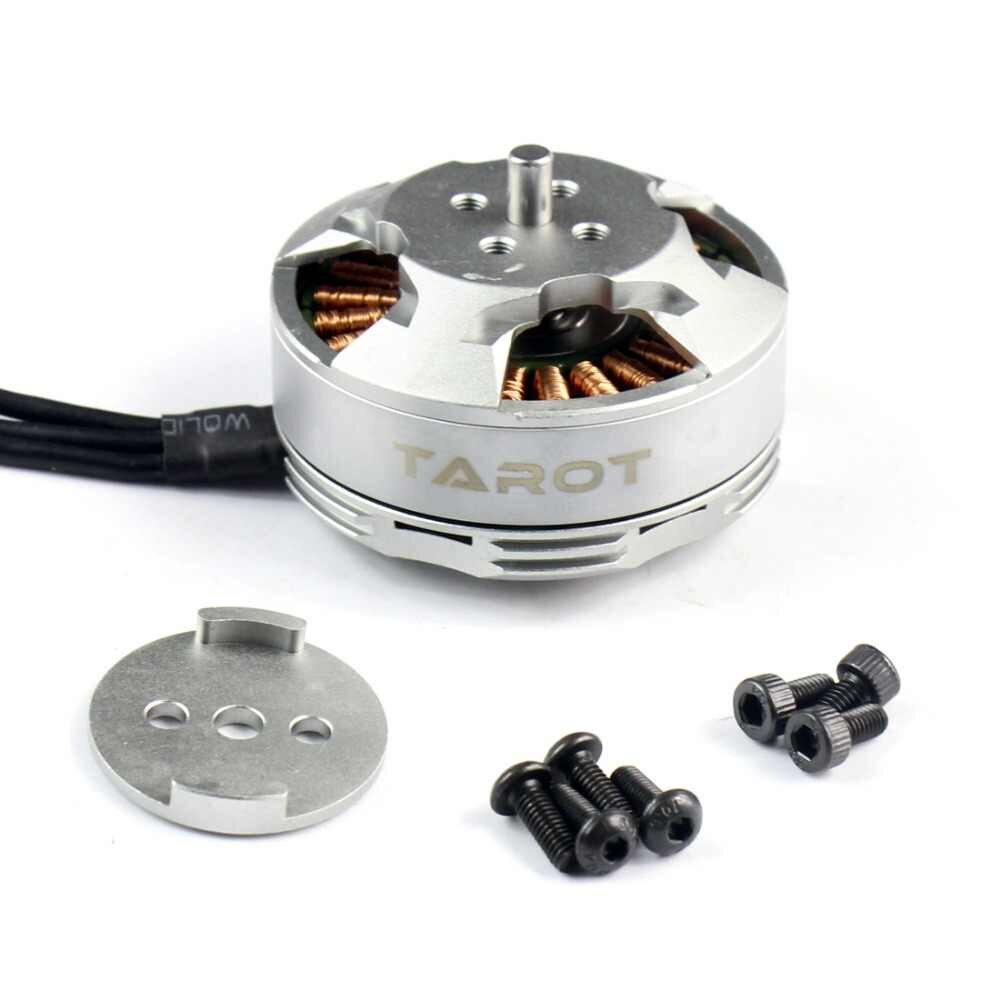
\includegraphics[width=\textwidth]{images/tarot_4108.jpg}
    %         \caption[The Tarot 4108 brushless electric motor.]{The Tarot 4108 brushless electric motor.\footnotemark}
    %         \label{subfig:tarot_4108}
    %     \end{subfigure}
    %     \hspace{2cm}
    %     \begin{subfigure}[b]{0.3\textwidth}
    %         \centering
    %         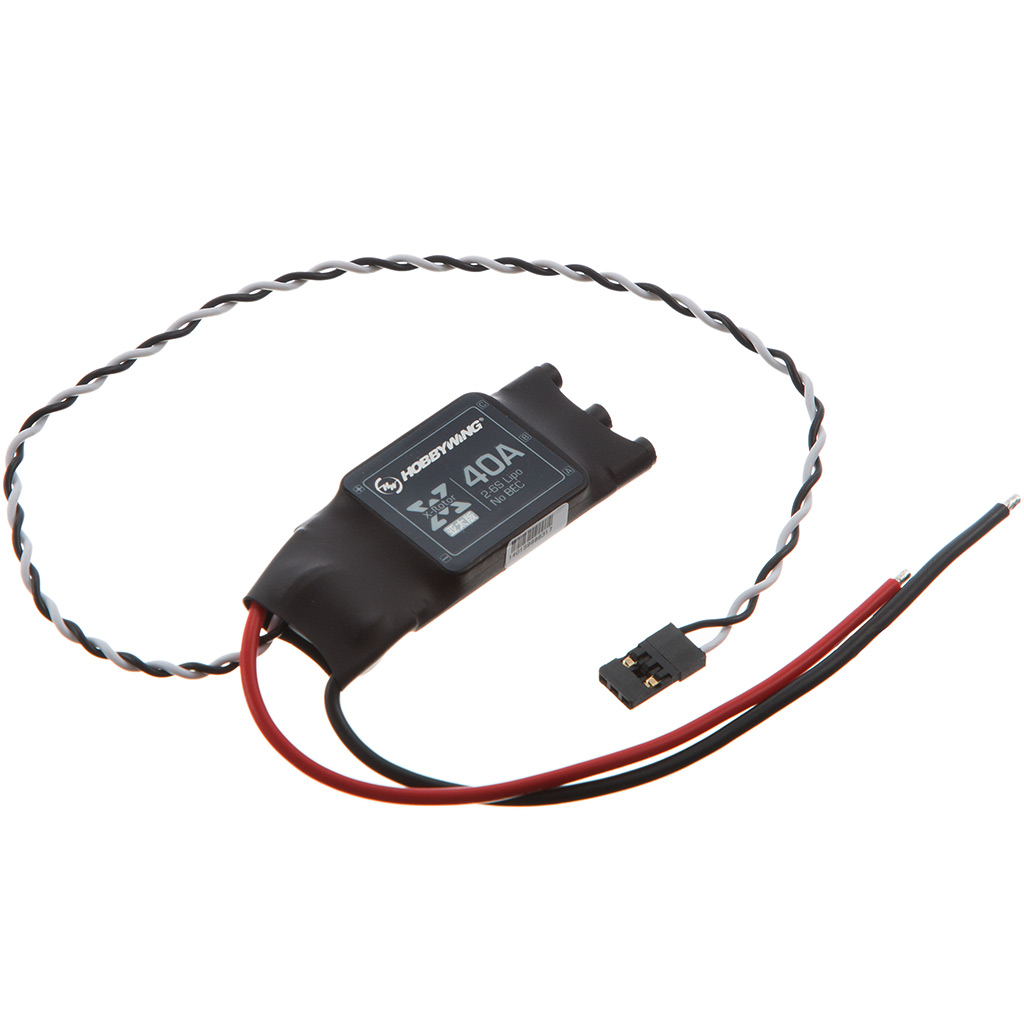
\includegraphics[width=\textwidth]{images/xrotor_40.jpg}
    %         \caption[The XRotor 40 A Speed Controller.]{The XRotor 40 A Speed Controller.\footnotemark}
    %         \label{subfig:xrotor_40}
    %     \end{subfigure}
    %     \caption{The drone motors and speed controllers.}
    %     \label{subfig:motors_and_speed_controllers}
    % \end{figure}
    % \footnotetext[2]{Image source: \url{https://www.aliexpress.com/i/32591702396.html}}
    % \footnotetext{Image source: \url{http://www.helipal.com/hobbywing-xrotor-40a-esc.html}}

    \item \textbf{Batteries:} Specific batteries have not been selected. The constraints for selection of batteries come from the selected power components and recommendations for the model. The battery should be a 22.2 V lithium-polymer battery with a capacity of about 10,000 mAh and a continuous discharge rate of at least 20 C. A smaller, 12.6 V battery should supply the flight controller and companion board with regulated power in order to isolate these computational components from transient effects caused by spikes in current draw by the motors.

\end{itemize}

\subsection{Flight Controllers}
\label{section:flight_controllers}

Multiple flight controller setups have been considered for this project. Each flight controller and the corresponding hardware setup have specific advantages and disadvantages, which are explained herein. The software architecture has been designed to accommodate multiple hardware architectures intrinsically, so that multiple hardware architectures may be compared (see Section \ref{subsection:landing_controller}).

% \subsubsection{Computational Hardware Requirements}
% The main considerations for hardware architecture are as follows:

% \begin{itemize}
%     \item \textbf{Minimalism} \\ The system needs to have as few components as possible, and as few cabled connections as possible. Necessary hardware connections should be properly secured.
%     \item \textbf{Physical robustness} \\ Hardware components should be securely fastened to the drone in a way that minimizes the effects of vibration and changing acceleration.
%     \item \textbf{Minimal power usage} \\ Hardware should be chosen such that it minimizes power usage, in order to reduce weight from necessary batteries, and prolong operational time.
%     \item \textbf{Maximum processing capability} \\ Hardware should provide more than adequate processing power for the tasks at hand, in order to provide reliability in flight.
%     \item \textbf{Maximum compatibility with existing software} \\ Hardware should be chosen which is compatible with necessary existing software, in order to minimize overhead caused by rewriting or adapting existing code and functionalities.
%     % \item \textbf{Demonstrated reliability} \\ Hardware must be proven and well-tested in order to provide reliability.
% \end{itemize}

% \noindent
\subsubsection{Multiple computational hardware setups will be tested:}

\begin{itemize}
    \item \textbf{Navio2 with Raspberry Pi 3 B+} \\ The Navio2 is a Raspberry Pi-targeted hat that provides \gls{IMU}, \gls{GPS}, \gls{UART}, \gls{ADC}, \gls{I2C}, and \gls{PWM} interfaces adequate for controlling drone hardware. It is shown connected to a Raspberry Pi 3 B+ in figure \ref{subfig:navio2_rpi_3}. The Navio2 is designed to run the ArduPilot software and has a corresponding \texttt{waf} board configuration. This is the de facto default setup when running ArduPilot on a Linux computer. The advantages of this setup are that it is extensively tested and relatively easy to extend, in that the Raspberry Pi has multiple USB ports and a camera interface with a specially-designed camera module for computer vision functions. \gls{ROS} is also tested for Raspberry Pi and the Raspbian operating system. The disadvantages of this setup are that the limited processing power of the Raspberry Pi must be shared between the ArduPilot process, the \gls{ROS} processes, and the standard Raspbian processes. This is a concern because the ArduPilot and \gls{ROS} processes must run in near real-time - that is to say, without delays. A possible workaround to this issue is to assign specific cores to the ArduPilot and \gls{ROS} processes respectively. However, the vision processing involved with detecting the landing pad's fiducial marker(s) can be processor-intensive. Any graphics processing or neural network processing could potentially be exported to a Google Coral Accelerator via USB. While this would add valuable processing power, it would also complicate the system by adding more points of failure in an environment subject to vibration and acceleration.
    \item \textbf{Pixhawk 2 Cube} \\ In the case that configuring the Google Coral Dev or NVIDIA Jetson Nano for the Navio2 is infeasible (shown hereafter), these will be used as companion boards for the Pixhawk 2 Cube. The Pixhawk will run ArduPilot on its own and be connected via USB or UART to the companion board, with minor changes to the software configuration, but no changes to the software architecture. The extra board does make the hardware system somewhat more complex, but provides more reliability in that the ArduPilot software will be the sole program running on the board. The companion boards in this scenario will run only the necessary ROS modules to carry out the image processing for the fiducial markers, generate the necessary coordinate system transforms, control the gimbal, and send velocity control messages to ArduPilot on the Pixhawk.
    % \begin{figure}[ht]
    %     \centering
    %     \subfloat[Raspberry Pi 3 B+ with Navio2 hat.\label{subfloat:navio2_rpi_3}]{ 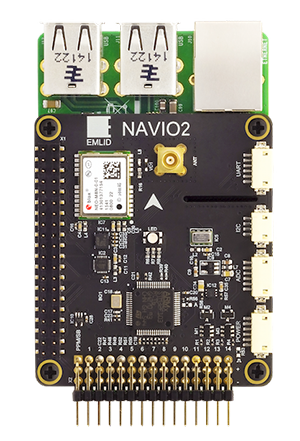
\includegraphics[angle=90,width=0.4\textwidth]{images/navio2_rpi3.png} } % https://docs.emlid.com/navio2/img/Navio2WithPaspberryPi.png
    %     \hspace{2cm}
    %     \subfloat[Google Coral USB Accelerator\label{subfloat:coral_usb}]{ 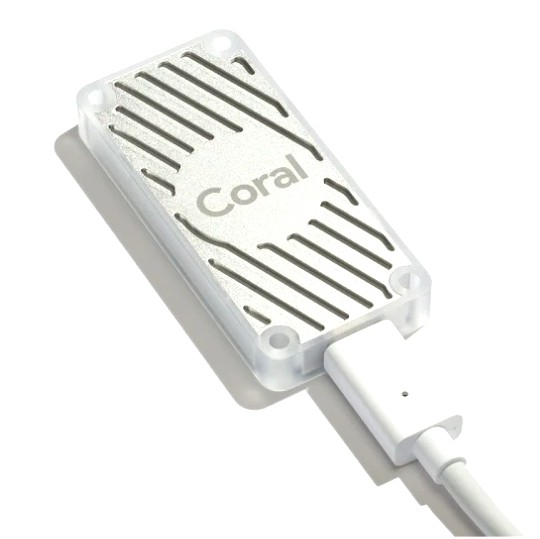
\includegraphics[width=0.3\textwidth]{images/coral_usb.jpg} } % https://cdn.antratek.nl/media/product/4a4/google-coral-usb-accelerator-114991790-796.jpg
    %     \label{fig:navio2_rpi3_coral_usb}
    % \end{figure}
    
    \begin{figure}[ht]
        \centering
        \begin{subfigure}[b]{0.3\textwidth}
            \centering
            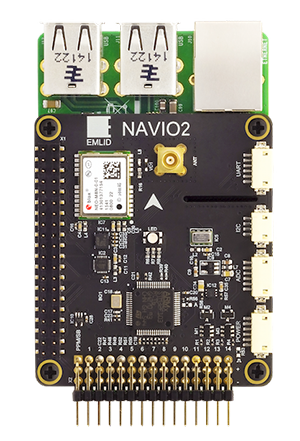
\includegraphics[angle=90,width=\textwidth]{images/navio2_rpi3.png}
            \caption[Raspberry Pi 3 B+ with Navio2 hat.]{Raspberry Pi 3 B+ with Navio2 hat.\footnotemark}
            \label{subfig:navio2_rpi_3}
        \end{subfigure}
        \hspace{1cm}
        % \begin{subfigure}[b]{0.4\textwidth}
        %     \centering
        %     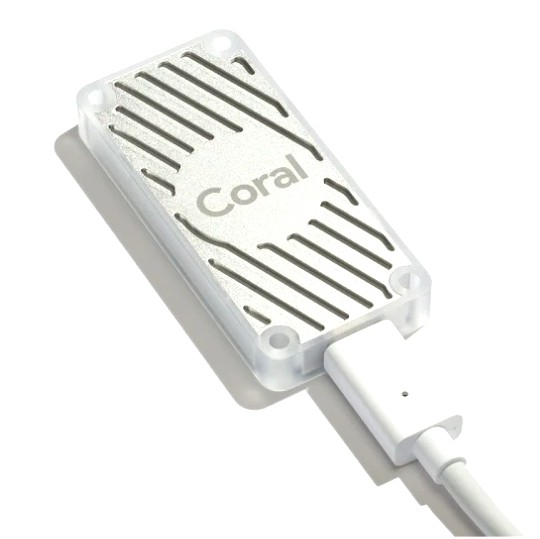
\includegraphics[width=\textwidth]{images/coral_usb.jpg}
        %     \caption[Google Coral USB Accelerator.]{Google Coral USB Accelerator.\footnotemark}
        %     \label{subfig:coral_usb}
        % \end{subfigure}
        % \begin{minipage}[b]{0.875\textwidth}
        % \vspace{0.25cm}
        % \caption{A possible system architecture comprised of a Raspberry Pi 3 B+, Navio2 hat, and Google Coral USB Accelerator.}
        % \end{minipage}
        % \label{fig:navio2_rpi3_coral_usb}
        \begin{subfigure}[b]{0.3\textwidth}
            \centering
            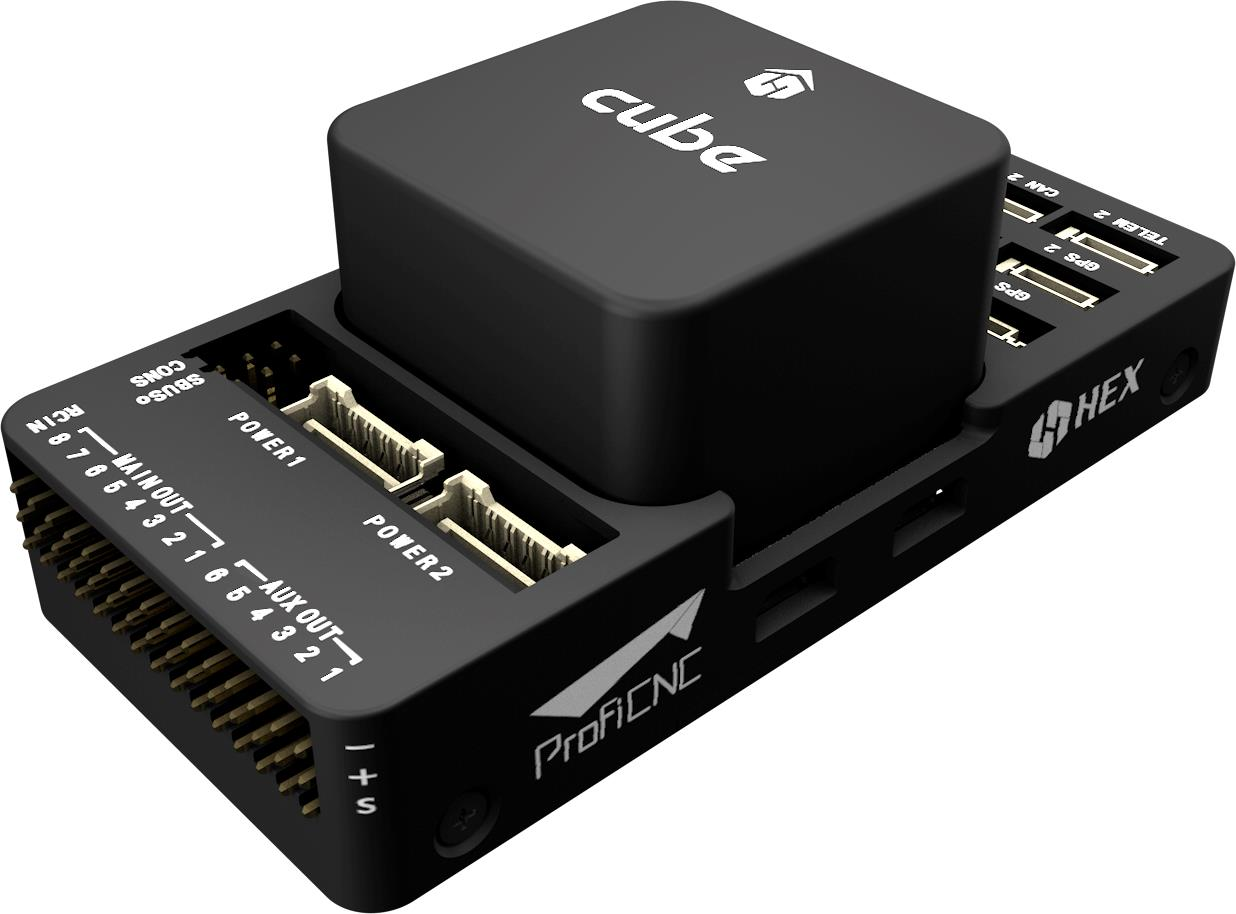
\includegraphics[width=\textwidth]{images/pixhawk2_cube_hero.png}
            \caption[The Pixhawk 2 Cube Hero]{The Pixhawk 2 Cube Hero\footnotemark}
            \label{fig:pixhawk_2_cube_hero}
        \end{subfigure}
    \end{figure}
    \footnotetext[2]{Image source: \url{https://docs.emlid.com/navio2/img/Navio2WithPaspberryPi.png}}
    \footnotetext[3]{Image source: \url{https://docs.px4.io/v1.9.0/en/flight_controller/pixhawk-2.html}}
    % \subfloat[QR Code]{{
\includegraphics[width=0.2\textwidth]{images/qr_code_example.png} }}
    
    \item \textbf{Navio2 with Google Coral Dev} \\ Google's Coral Dev board (shown in figure \ref{subfig:coral_dev}) is similar to the Raspberry Pi in its form but also features Google's Edge \gls{TPU}, which allows for much faster graphics and neural network processing than that of the Raspberry Pi and similar boards. It also has a camera port and specially-designed camera module, but only a single USB port. The advantage of the Google Coral Dev is that the image processing and any potential neural network processing could be exported to the \gls{TPU} for faster processing, keeping the load on the CPU significantly lower. Since the Navio2 is developed for the Raspberry Pi specifically, some effort will be required to configure the boards to work together.
    
    \item \textbf{Navio2 with NVIDIA Jetson Nano} \\ NVIDIA's Jetson Nano is similar to the Raspberry Pi and Google Coral Dev Boards. It uses the Raspberry Pi camera module, has an onboard GPU and is also targeted to embedded artificial intelligence and neural network applications. The image processing for the fiducial markers would be exported to the GPU as much as possible. It, like the Google Coral, is theoretically compatible with the Navio2 after some configuration. 

    \footnotetext[4]{Image source: \url{https://www.aliexpress.com/item/33025840366.html}}
    \footnotetext[5]{Image source: \url{https://developer.nvidia.com/embedded/jetson-nano-developer-kit}}
    % \footnotetext[5]{Image source: \url{https://www.antratek.com/coral-usb-accelerator}}

    \begin{figure}[h!]
        \centering
        \hspace{2cm}
        \begin{subfigure}[b]{0.3\textwidth}
            \centering
            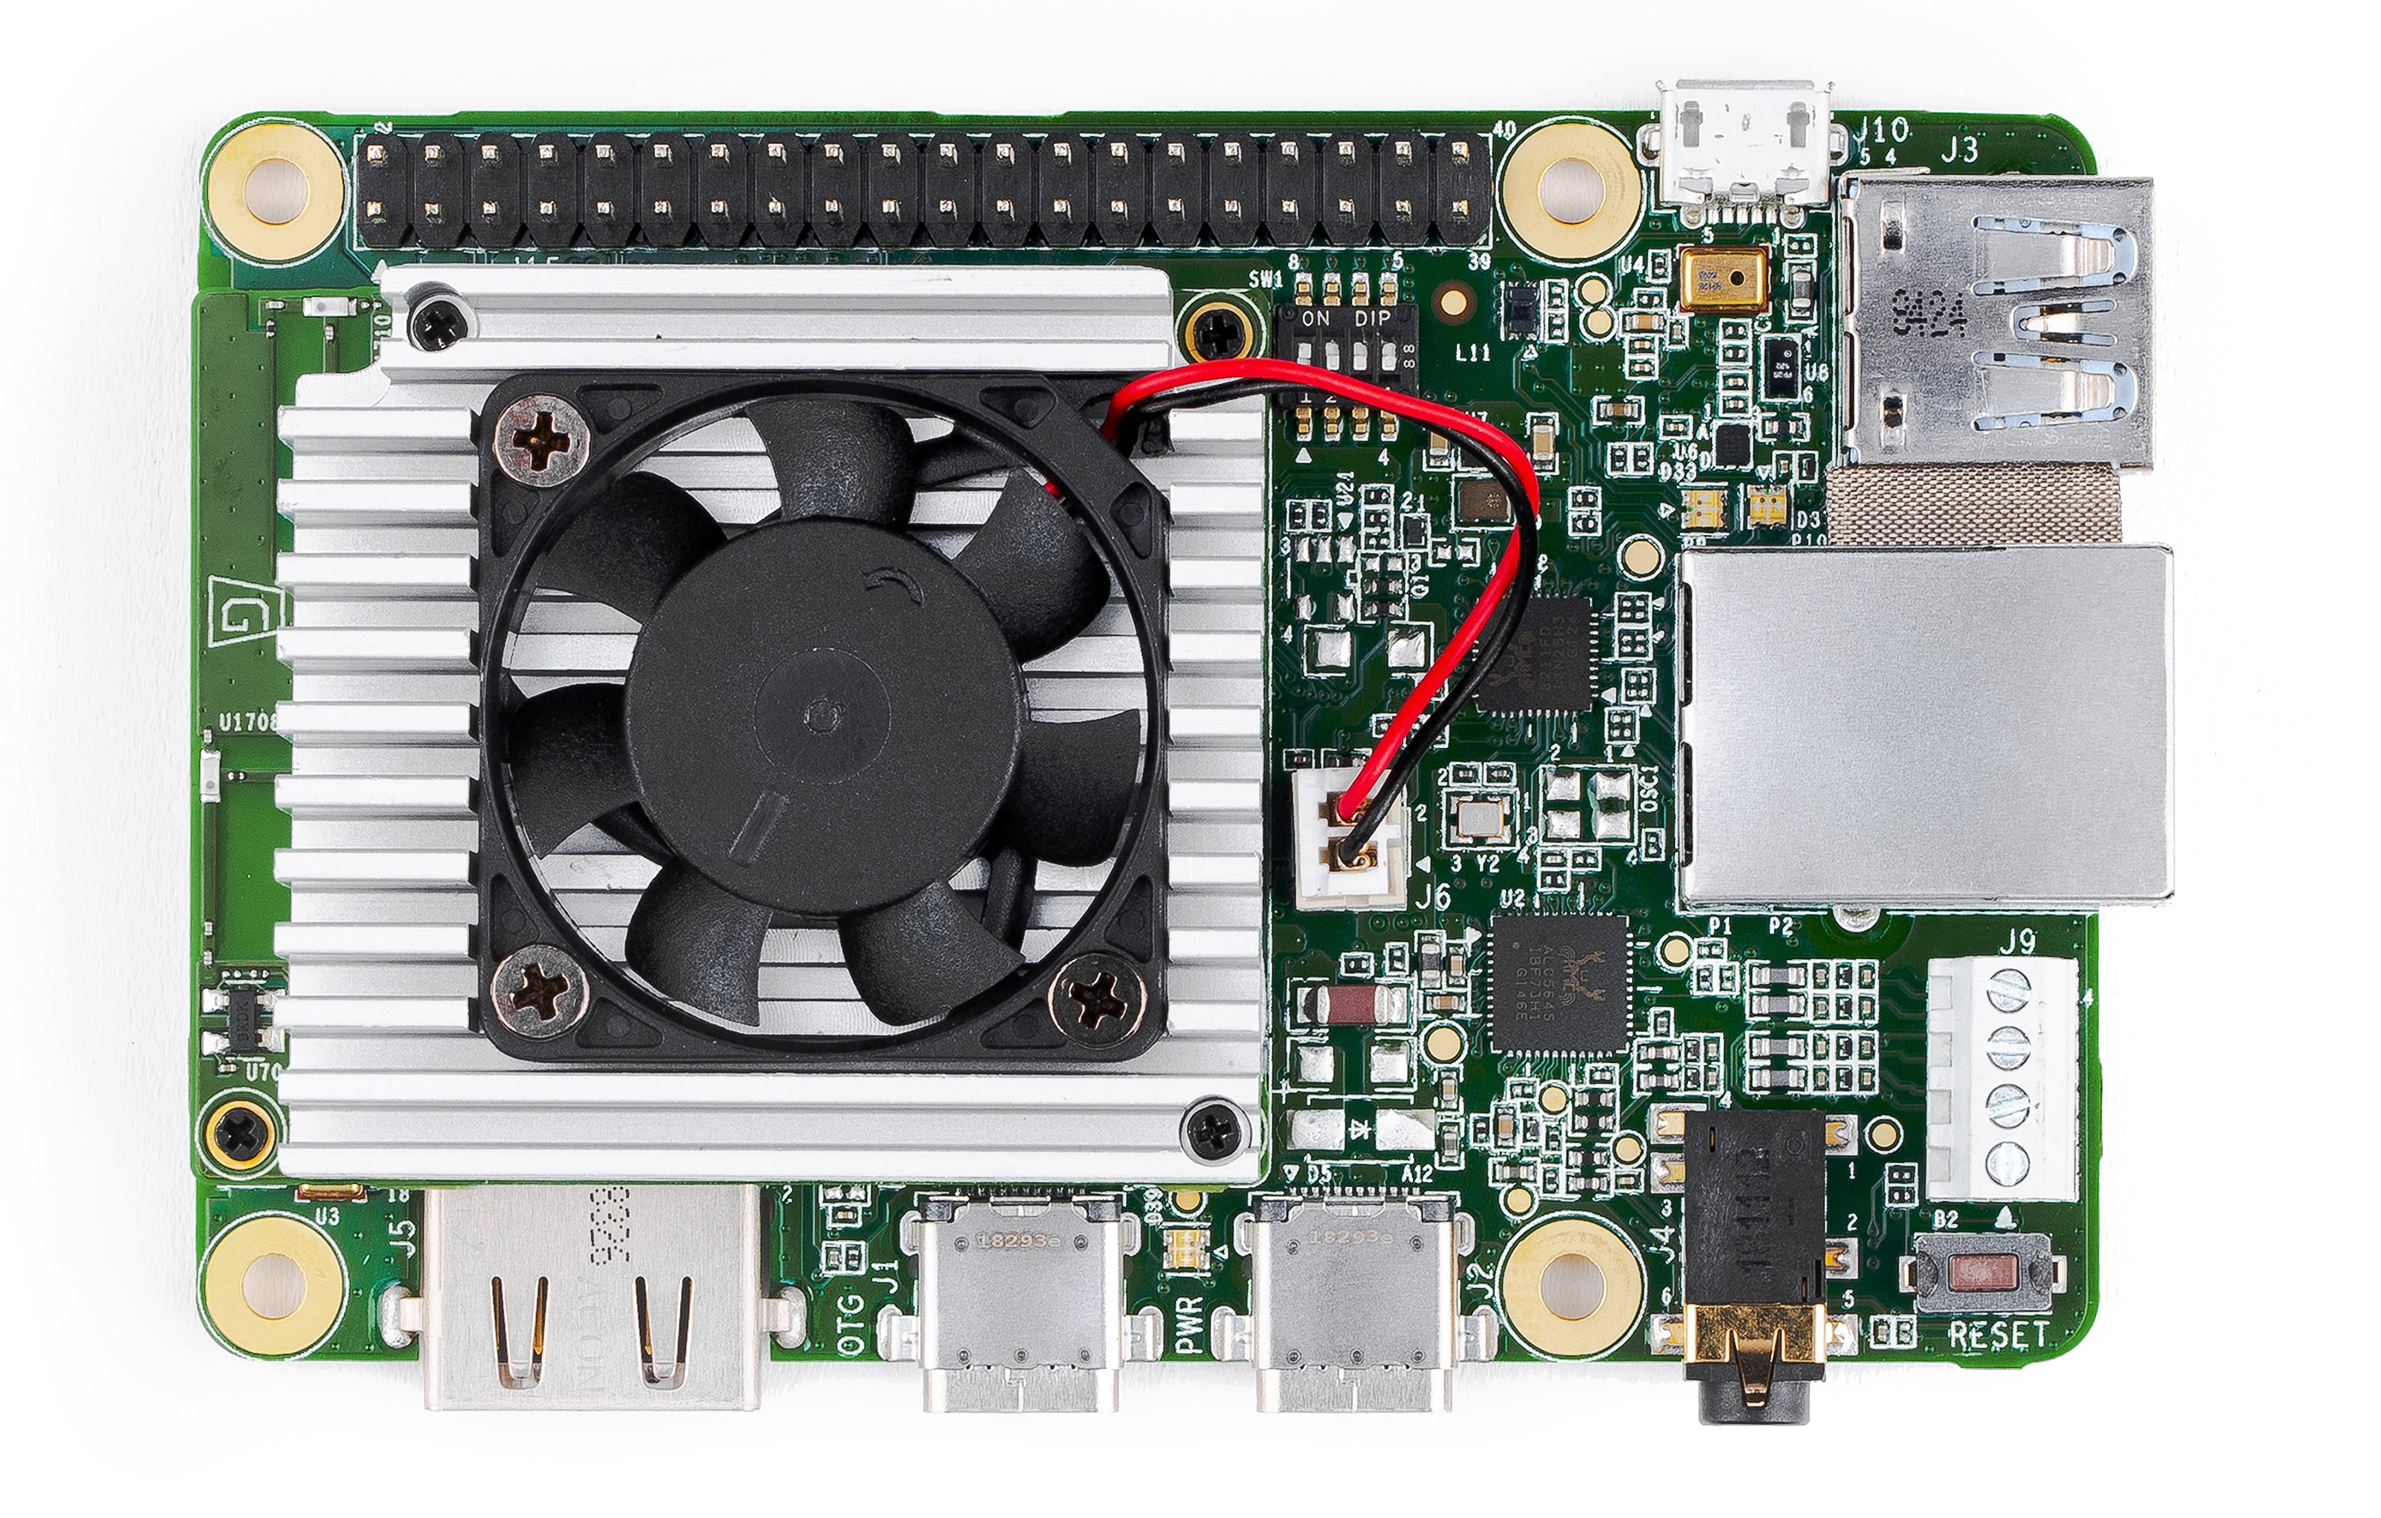
\includegraphics[width=\textwidth]{images/coral_dev.jpg}
            \caption[Google's Coral Dev Board]{Google's Coral Dev board.\footnotemark}
            \label{subfig:coral_dev}
        \end{subfigure}
        \hspace{1cm}
        \begin{subfigure}[b]{0.3\textwidth}
            \centering
            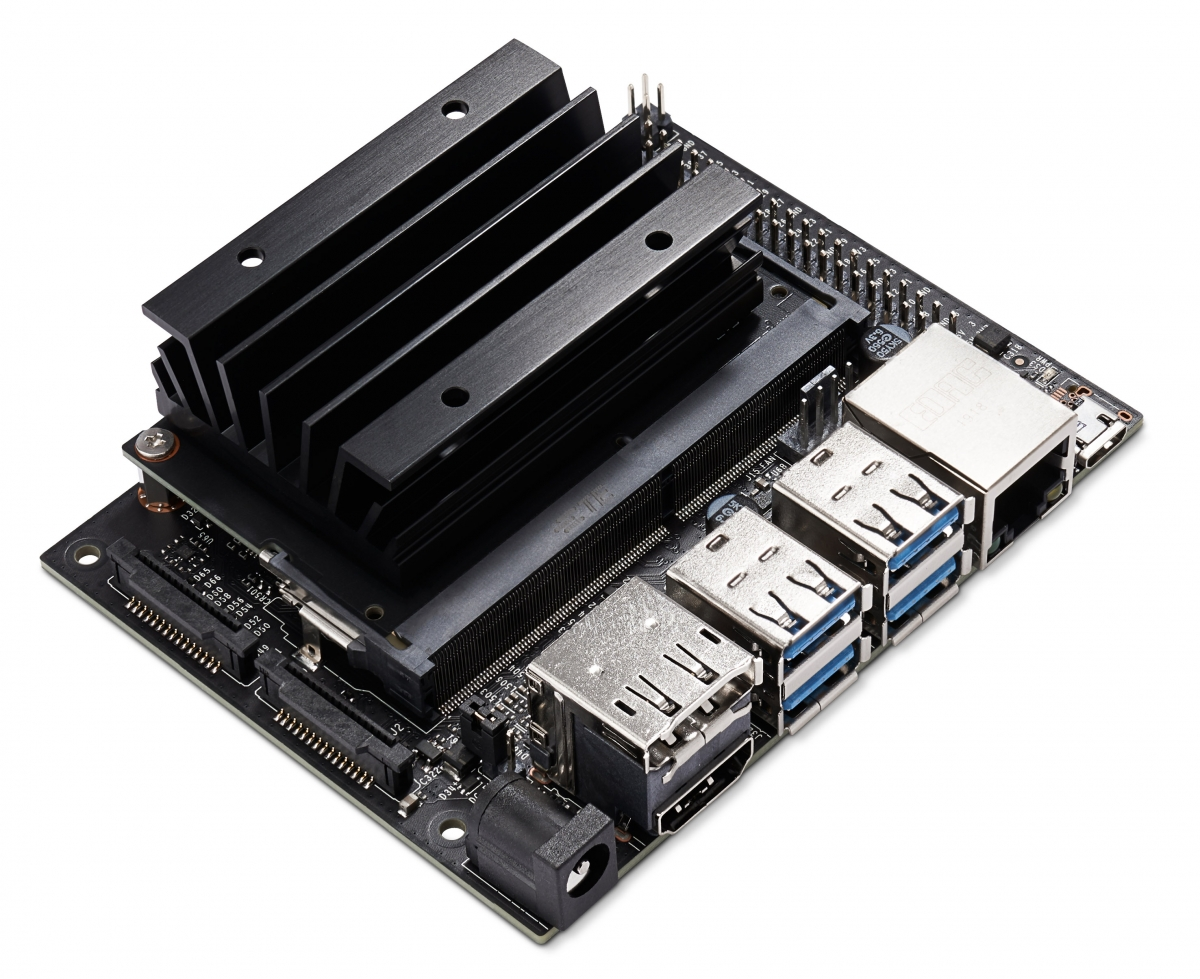
\includegraphics[width=\textwidth]{images/nvidia_jetson_nano.jpg}
        \caption[The NVIDIA Jetson Nano Dev board.]{NVIDIA Jetson Nano.\footnotemark}
        \label{subfig:nvidia_jetson_nano}
        \end{subfigure}
        \caption{The computationally stronger companion boards.}
        \label{fig:companion boards}
    \end{figure}
    

    

    
    % \begin{figure}[ht]
    %     \centering
    %     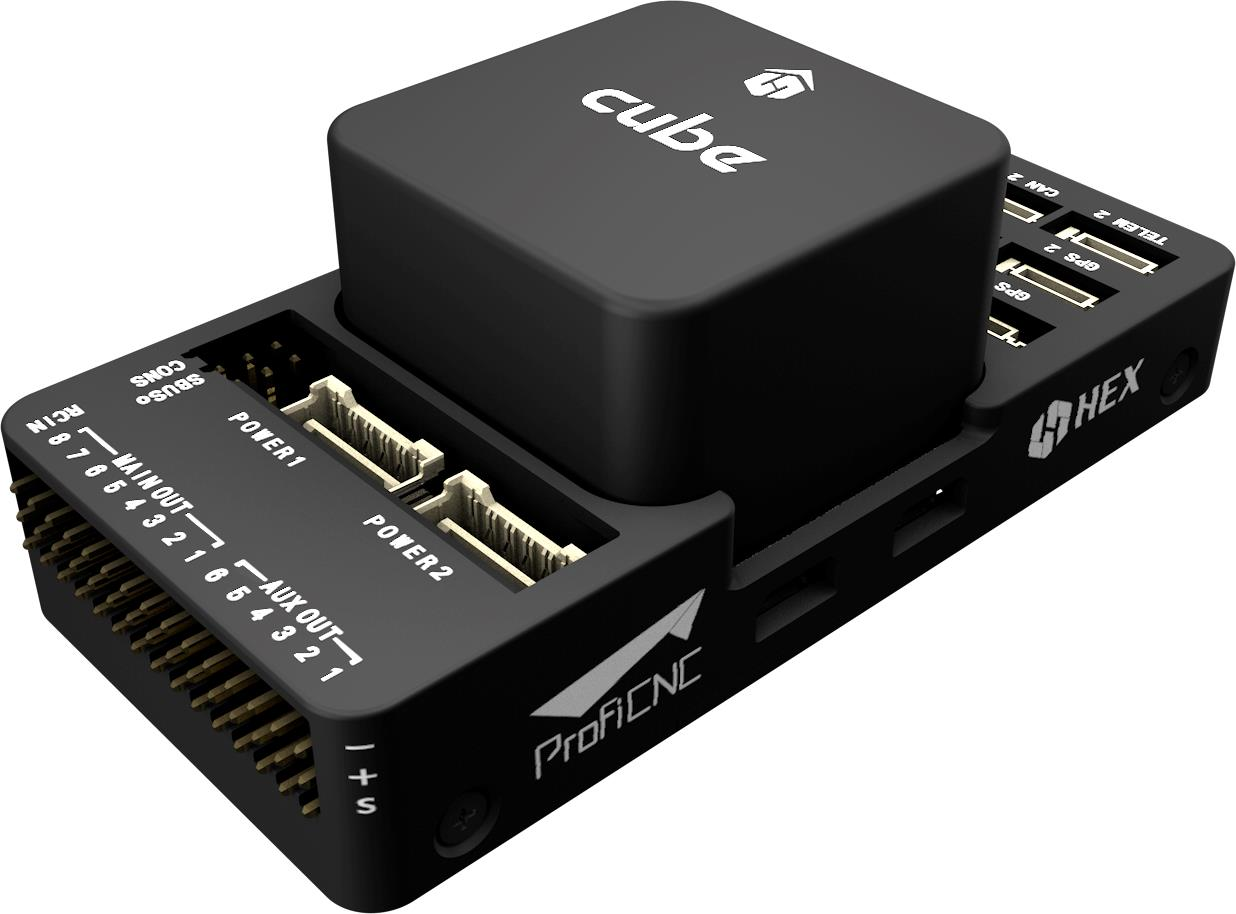
\includegraphics[width=0.35\textwidth]{images/pixhawk2_cube_hero.png}
    %     \caption[The Pixhawk 2 Cube Hero]{The Pixhawk 2 Cube Hero\footnotemark}
    %     \label{fig:pixhawk_2_cube_hero}
    % \end{figure}

\end{itemize}



% \section{\color{red}Migration from Simulator to Hardware}

% {\color{red}The landing system itself is usable both in the simulator and on a real hardware system. Some specifics will need to be changed to suit the particular system, including certain ROS topics, data sources, PID gains, etc. A basic framework for migrating this software from the simulator to a hardware system is as follows:
% \begin{itemize}
%     \item Camera calibration using the chessboard framework as in Section 3.1
%     \item Tuning of the gimbal controller system and adaptation of the PID controller system to the specific gimbal. This will require extraction of yaw and pitch (and possibly roll) values from the gimbal's IMU, or possibly more accurate step-based method of tracking the gimbal's position over time.
%     \item Construction of the drone as a purely radio-controlled model.
%     \item Tuning of the drone's onboard PID systems and other parameters for reliable, smooth control.
%     \item Determination of the gimbal's acceptable range of motion, and integration of this range of motion into the gimbal controller.
%     \item Calibration of the fiducial marker systems in a truly stationary setting, i.e. pose estimation while the drone is sitting perfectly still and the marker is being moved from location to location.
%     \item Stationary, in-flight testing of pose estimation accuracy using all relevant fiducial markers.
%     \item Application of sensor fusion and filtering to in-flight pose estimation and subsequent re-testing.
%     \item Addition of mode-switch using an RC switch so that a pilot can switch to landing mode but take control easily at any time.
%     \item Gradual testing of the setpoint\_raw functionality in mavros. First this should be tested without the z-axis. The drone should follow the landing pad while maintaining its initial altitude. This should be done both with stationary and moving landing pads. Then the drone's descent should be tested on a stationary landing pad. Then on a moving landing pad.
% \end{itemize}
% }